\section{Restaurant}
The robots are tested in a real environment such as a real restaurant or a shopping mall.
There are \emph{two} robots helping clients in the restaurant at the same time.

\subsection{Focus}
This test focuses on online mapping, safe navigation in previously unknown environments, gesture detection, human-robot interaction, and manipulation in a real environment.

The robot will need to create its own map from the environment and then move within it to handle human requests, such as delivering drinks or snacks, while people are walking around.
As this test is performed with 2 robots in parallel, the robots will also have to avoid each other. 

\subsection{Setup}
\begin{enumerate}
	\item \textbf{Location:} A real restaurant fully equipped with a \quotes{Professional Barman} i.e. the operator and at least three tables with \quotes{Professional Clients}. 
\end{enumerate}

\subsection{Task}
\begin{enumerate}
	\item \textbf{Start:} The robot starts at a designated starting position. After the start signal is given, the robot may look around to keep an \textit{eye} on the tables.
	  The location of the tables is not taught to the robot via some training phase. 
	
	\item \textbf{Calling:} A guest will ask for the robot's attention by waving \emph{and} calling it out using voice. 
	  The robot must state out loud that it has detected the call.
	  % A robot must also indicate roughly where it has detected the call (e.g. \quotes{to my left})
	  In case both robots notice the same call, the \textit{Professional Barman} will tell one of the robots to take the order. 
	  The barman will say the robot's name followed by \quotes{Take the order} e.g. \quotes{R2D2, take the order}. 
	  The other robot will simply have to wait for another call. 
	  If the robot \textit{not} commanded to take the order still goes, it will be commanded to wait (e.g. \quotes{C3PO, Wait}). 
	  In case the robot keeps going after that, the emergency button will be used to stop the robot. 
	
% 	\item \textbf{Parallel orders:} It may occur that two guests want to order something at the same time and thus wave at the same time. 
% 	  The referees will arange these two guests such that each is clearly visible to (in front of) one of the robots. 
	
	\item \textbf{Ordering}: The robot must ask the person what he or she wants to order. See Orders below for details about ordering.
	\item \textbf{Avoiding random person:} At any time while going to any of the tables or to the \textit{Kitchen}, a person may step on the robot's path. 
	  It is expected of the robot to avoid that person or stop and wait for it to move away.

	\item \textbf{Delivering phase:}
	\begin{enumerate}
		\item \textbf{Repeating the order:} Once again in the kitchen, the robot recites the orders for each table (e.g.~\textit{\quotes{Hamburger with fries for table A and Orange juice for table B}}, to the \textit{Professional Barman}. 
		  The \textit{Professional Barman} will serve the order and place it into a tray on the Kitchen-bar.
		  If the barman cannot understand the order that the robot repeats, he cannot hand out the order and no points can be awarded for reciting the order.

		\item \textbf{Grabbing a beverage:} The robot must grab a can of the appropriate drink from a set of cans on the Kitchen-bar. 

		\item \textbf{Grabbing a combo:}  The robot must carry a tray with the ordering from the kitchen-bar. 
		Teams must indicate beforehand whether the robot is able to grasp the plate itself, whether it needs a tray or whether the plate needs to be handed to the robot.
		
		\item \textbf{Delivery:} The robot must place the order on the table. 
		If the robot is not able to do this, the robot is allowed to hand over the order, but the client is not allowed to shift his/her chair or stand up. 
		The robot must help the client, not the other way around. 
	\end{enumerate}
	
	\item \textbf{Next customer, please:} When the robot is in the kitchen, the \textit{Professional Barman} will ask the robot to either find a new client to serve or to stop the test.
	The barman will either tell the robot \quotes{R2D2, Wait} to make it wait for another client or \quotes{R2D2, Stop the test} to end the test for that robot. 
\end{enumerate}

\textbf{Orders:} The menu offers Beverages and Combos. An order may be a Beverage or Combo. Some guest(s) will order a Combo while another will order a Beverage.
  A Combo is a combination of two of the food items from the set of objects \ref{rule:scenario_objects}, e.g. \quotes{noodles with peanuts} or \quotes{noodles and peanuts}. 
  Guests also prefer to state their order in a natural way, as they would in a restaurant operated by humans.
  
\begin{figure}[tbp]
	\centering
	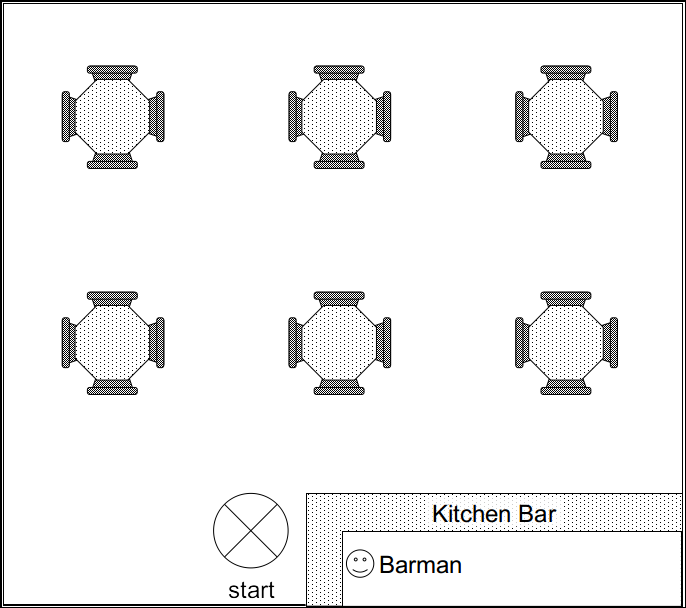
\includegraphics[width=0.5\columnwidth]{images/restaurant.png}
	\caption{Restaurant test: example setup.}
	\label{fig:restaurant}
\end{figure}

\subsection{Additional rules and remarks}

\begin{itemize}
	\item \textbf{Safety!} This test takes place in a public area. That is, there may be people standing, sitting or walking around the area throughout the test. The robot is expected to not even slightly touch anything and is immediately stopped in case of danger.

	\item \textbf{Referees and guidance:} For safety reasons, the referees in this test are TC members. One of the referees follows the robot and is always in reach of the emergency button.

	\item \textbf{Start:} There is no fixed start signal in this test, it starts when both robots are ready (though within a reasonable time).

	\item \textbf{Order:} The way the user provides information to the robot is up to the robot's team. A natural interaction is preferred.

	\item \textbf{Location:} This test can be arranged in any real restaurant or shopping mall. If this is not possible, the test can be conducted in an arbitrary room containing the appropriate locations. 
	  The only requirement is that this room is not part of the arena and that the teams do not know the room beforehand. 
	  The exact location, including the object and delivery locations, will be defined by the technical committee on site (and in corporation with the local organization). 
	  In addition, to avoid unnecessary time investment for navigation, the distances between tables and the \quotes{Kitchen Bar} will be minimal.

	\item \textbf{Disturbances from outside:} If a person from the audience (severely) interferes with the robot in a way that makes it impossible to solve the task, the teams may repeat the test immediately.

	\item \textbf{Learning tables:} Of course, it can only be sure that a robot correctly remembered where an order is suppposed to be delivered when it is able to go there after grabbing the order. 
	
	\item \textbf{Instruction:} The robot interacts with the operators, not the team. That is, the team is only allowed to (very!) briefly instruct the \textit{Professional Barman} 
	\begin{itemize} 
		\item How to the tell the robot the order has been served
	\end{itemize}
	It is not allowed to the team to instruct the clients on how to get robot's attention. It shall be done in a natural way like when interacting with a human waiter.

	\item \textbf{Kitchen-bar:} The \textit{Kitchen-bar} will be a table located at the restaurant's kitchen, next to the place where the robot started. 
	The robot may ask on which side of the robot the Kitchen-bar is, e.g. on its left or right side. It may ask this at any time, but it is better if the robot infers this itself. 
	It has the following setup.
	\begin{itemize}
		\item \textbf{Barman:} A \textit{Professional Barman} (member of the TC) will be at the other side of the Kitchen-bar to take the order provided by the robot and serve it in the official tray.
		\item \textbf{Beverages:} Beverages will be located on the Kitchen-bar next to the \textit{Professional Barman}.
	\end{itemize}

\end{itemize}

\subsection{Data recording}
  Please record the following data (See \refsec{rule:datarecording}):
  \begin{itemize}
   \item Audio
   \item Commands
   \item Mapping data
   \item Images
   \item Plans
  \end{itemize}

\subsubsection{Referee instructions}

The referee needs to
\begin{itemize}
  \item Prepare orders for each client in advance, so that there can be no confusion. These orders must also be available at the kitchen. 
\end{itemize}

% \subsubsection{OC instructions}

% \textbf{2 hours before the test}
% \begin{itemize}
% \item 
% \item 
% \end{itemize}
% \textbf{During the test}
% \begin{itemize}
% \item 
% \item 
% \end{itemize}

\newpage
\subsection{Score sheet}
The maximum time for this test is 15 minutes.

\small\begin{scorelist}

	\scoreheading{Training phase}
	\scoreitem[3]{10}{Learning the location of a table (Professional Waiter)}
	\scoreitem[3]{5}{Learning the location of a table (Custom Waiter)}
	\scoreitem[3]{10}{Inferring the side on which a table is (Professional Waiter only)}
	
	\scoreheading{Ordering phase}
	\scoreitem{5}{Understanding which table to take an order from}
	\scoreitem{15}{Going to the designated table}
	\scoreitem{10}{Taking an order from the designated table}
	\scoreitem{20}{Noticing a waving/calling person from distance}
	\scoreitem{20}{Going to the table of the waving/calling person}
	\scoreitem{10}{Taking an order from the waving/calling person}
	\scoreitem{10}{Avoiding a person crossing the robots' path}

	\scoreheading{Delivering phase}
	\scoreitem[2]{5}{Reciting both the order and table number for both tables}
	\scoreitem{10}{Grasping the correct drink}
	\scoreitem{15}{Getting close to the correct table with the drink}
	\scoreitem{15}{Delivering the drink by placing it on the correct table}
	\scoreitem{15}{Picking up the plate}
	\scoreitem{15}{Getting close to the correct table with the plate}
	\scoreitem{20}{Delivering the plate by placing it on the correct table}

	\setTotalScore{250}
\end{scorelist}



% Local Variables:
% TeX-master: "Rulebook"
% End:


% Local Variables:
% TeX-master: "Rulebook"
% End:
